\section{Modulation vom Tag zum Lesegerät}
Nach dem Aufbau des Tags wurde die Kommunikation zwischen Lesegerät und RFID-Tag betrachtet. Ziel ist es, die Lastmodulation des Tags sichtbar zu machen und das entstehende demodulierte Signal am Ausgang des Lesegeräts zu untersuchen.

\subsection{Schaltung}
Die Gesamtschaltung besteht aus dem Lesegerät in \cref{fig:lesegeraet_modulation_schaltung} und der Modulationsstufe des Tags in \cref{fig:tag_modulation_schaltung}. Das Lesegerät erzeugt über den Übertrager das magnetische Feld und wertet über den Hüllkurvendetektor die durch den Tag verursachten Feldänderungen aus.

Am Tag wird dazu ein Rechtecksignal angelegt, das den Lasttransistor periodisch ein- und ausschaltet. Dadurch ändert sich die Belastung des Resonanzkreises. Diese Laständerung wirkt sich auf das Feld des Lesegeräts aus und kann dort nach dem Hüllkurvendetektor gemessen werden.

\begin{figure}[H]
  \centering
  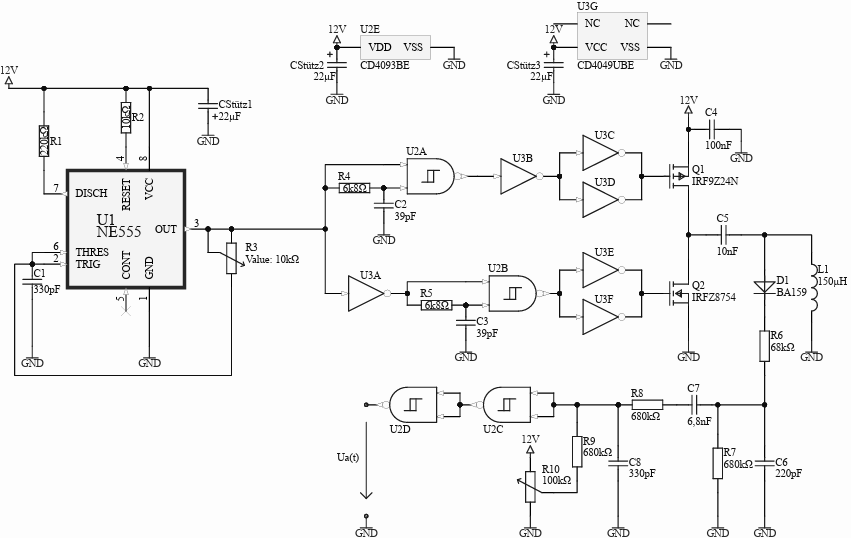
\includegraphics[width=0.8\linewidth]{Schaltungen/Lesegeraet_Modulation}
  \caption{Schaltung des Lesegeräts zur Demodulation}
  \label{fig:lesegeraet_modulation_schaltung}
\end{figure}

\begin{figure}[H]
  \centering
  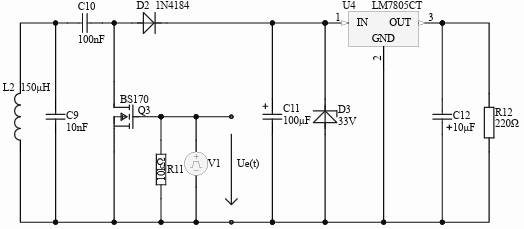
\includegraphics[width=0.6\linewidth]{Schaltungen/Tag_Modulation}
  \caption{Schaltung der Modulation am RFID-Tag}
  \label{fig:tag_modulation_schaltung}
\end{figure}

\subsection{Messvorgang}
Am Tag wird ein Rechtecksignal angelegt, das die Lastmodulation ansteuert. Als Anregung wird ein TTL-Pulsgenerator mit einer Spannung von $5\,V$ und einer Frequenz von $500\,Hz$ verwendet. Gemessen wird danach am Lesegerät hinter dem Hüllkurvendetektor beziehungsweise Hüllkurvendemodulator mit dem Oszilloskop.

Dabei wird geprüft, ob das am Tag angelegte Rechtecksignal im demodulierten Verlauf am Lesegerät wieder erkennbar ist. Die Messung soll zeigen, dass die vom Tag verursachte Laständerung erfolgreich zum Lesegerät übertragen wird.

\subsection{Messergebnis}
In \cref{fig:modulation_sekundaerseite} ist auf CH1 das Eingangssignal und auf CH2 das modulierte Signal auf der Sekundärseite dargestellt.
 
In \cref{fig:modulation_primaerseite} ist wieder auf CH1 das Eingangssignal und auf CH2 das modulierte Signal auf der Primärseite des Lesegeräts zu sehen. In beiden Aufnahmen ist erkennbar dass sich die Laständerung des Tags auf die Übertrager auswirkt.

Besonders deutlich wird die Modulation in \cref{fig:modulation_ue_ua}. Dort ist auf CH1 das Eingangssignal $U_e(t)$ und auf CH2 das modulierte beziehungsweise demodulierte Ausgangssignal $U_a(t)$ zu sehen. Das am Tag angelegte Rechtecksignal erscheint nach der Demodulation als Ausgangssignal $U_a(t)$ am Lesegerät wieder. Der Verlauf des Ausgangssignals folgt dem angelegten Rechtecksignal und bestätigt damit die erfolgreiche Signalübertragung vom Tag zum Lesegerät.


\begin{figure}[H]
  \centering
  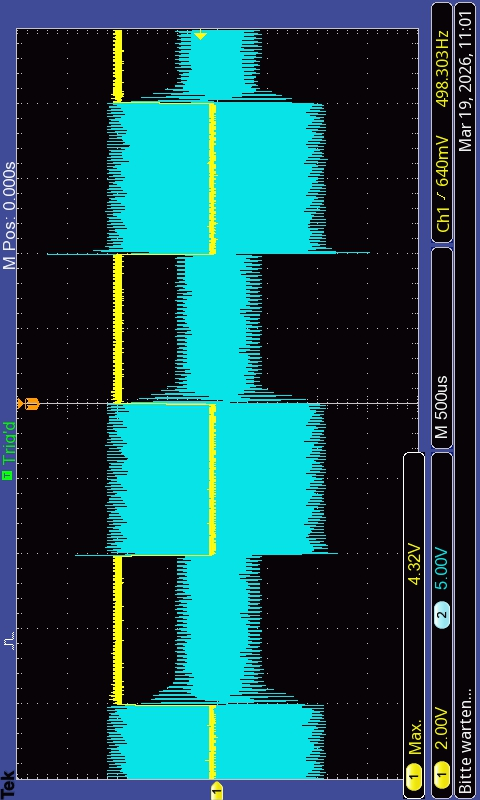
\includegraphics[width=0.42\linewidth, angle=-90]{Modulation_Tag--Lesegeraet/Ue_t_Sekundaerseite}
  \caption{Messung der Modulation auf der Sekundärseite}
  \label{fig:modulation_sekundaerseite}
\end{figure}

\begin{figure}[H]
	\centering
	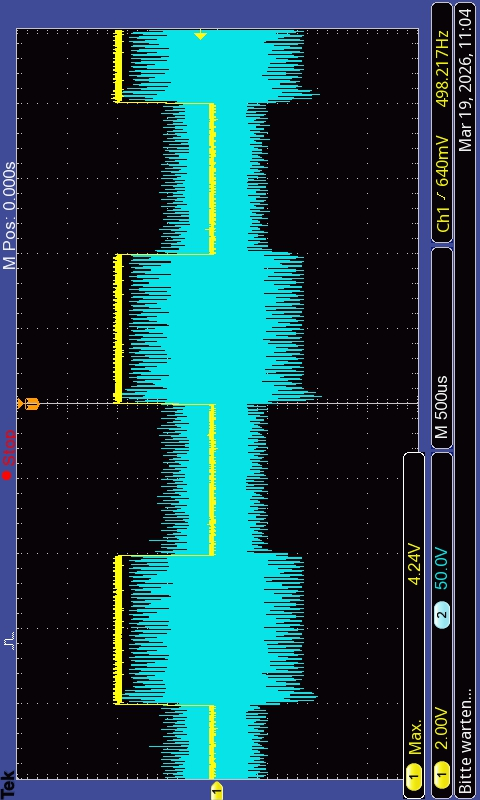
\includegraphics[width=0.42\linewidth, angle=-90]{Modulation_Tag--Lesegeraet/Ue_t_Primaerseite}
	\caption{Messung der Modulation auf der Primärseite}
	\label{fig:modulation_primaerseite}
\end{figure}

\begin{figure}[H]
  \centering
  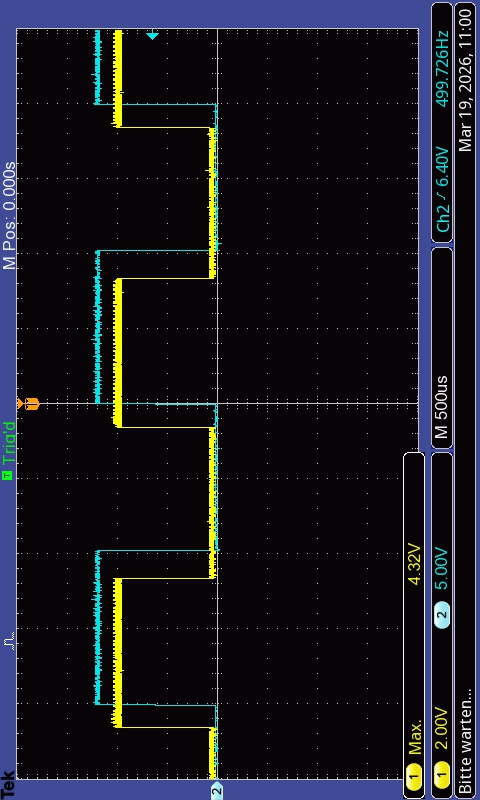
\includegraphics[width=0.42\linewidth, angle=-90]{Modulation_Tag--Lesegeraet/Ue_t_Ua_t}
  \caption{Vergleich von Eingangs- und Ausgangssignal der Modulation}
  \label{fig:modulation_ue_ua}
\end{figure}

\subsection{Interpretation}
Die Messung bestätigt das Funktionsprinzip der RFID-Kommunikation vom Tag zum Lesegerät. Der Tag sendet kein eigenes HF-Signal aus, sondern verändert durch Lastmodulation die Feldbelastung des Lesegeräts. Durch die Auswertung nach dem Hüllkurvendetektor kann diese Änderung sichtbar gemacht werden. Wird am Tag ein Rechtecksignal angelegt, so ist nach dem Hüllkurvendetektor am Lesegerät ein entsprechender Signalverlauf messbar.
